\chapter{PENDAHULUAN}
\pagenumbering{arabic}
\setcounter{page}{1}

Bab ini memaparkan latar belakang yang mendasari penulisan tugas akhir ini; rumusan masalah, tujuan, dan batasan tugas akhir secara formal; metodologi pengerjaan tugas akhir ini; dan sistematika pembahasan untuk bab-bab berikutnya pada laporan tugas akhir ini.

\section{Latar Belakang}

Studi di bidang robotika merupakan salah satu bidang riset dalam lingkup intelegensi buatan yang memiliki aplikasi yang sangat luas dalam kehidupan manusia. Perkembangan robotika telah memiliki dampak yang sangat besar dalam perkembangan zaman, terutama di bidang industri manufaktur dimana robot memungkinkan pekerjaan kompleks untuk dilakukan dengan volume tinggi. Secara umum, robotika telah maupun sangat berpotensi untuk membantu menciptakan peralatan otomatis yang dapat mengerjakan pekerjaan kompleks dengan akurasi, kecepatan, ketahanan, maupun tingkat keamanan yang lebih tinggi dibandingkan dengan manusia di berbagai bidang lainnya, seperti industri pertahanan, pertambangan, sampai industri kesehatan.

Dalam studi dan pengembangan robotika, peneliti mengkaji dan mempelajari bagaimana robot dapat direkayasa untuk menyelesaikan pekerjaan yang kompleks. Lingkup studi ini pun mencakup area yang luas, dari bagaimana robot dapat berinteraksi dengan manusia sampai bagaimana robot dapat berkoordinasi dengan banyak robot lainnya dalam menyelesaikan pekerjaannya. Sebagai sistem fisik siber, robot yang baik dapat melakukan persepsi dan membaca keadaan dunia dengan akurat, melakukan komputasi dan pengambilan keputusan tingkat tinggi, dan mengeksekusi suatu aksi dengan presisi.

\begin{figure}[h]
    \centering
    \medskip
    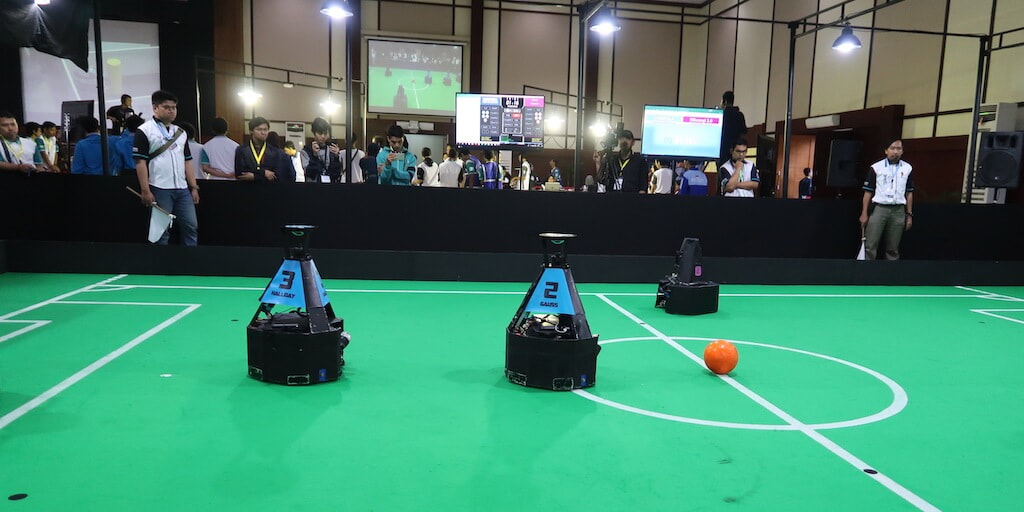
\includegraphics[width=0.8\textwidth]{resources/robotics-soccer.jpg}
    \caption{Tim DAGOZILLA pada Kontes Robot Indonesia}
    \label{fig:robotics-soccer}
    \bigskip
\end{figure}

Salah satu inisiatif untuk membangkitkan perkembangan di bidang robotika ini adalah liga pertandingan Robocup, yang merupakan liga pertandingan terbuka untuk tim pengembang dari universitas maupun organisasi lainnya untuk merekayasa robot-robot yang dapat ditandingkan antar tim. Diantara cabang liga yang ditandingkan dalam Robocup adalah kompetisi robot sepak bola beroda, dimana peserta mengembangkan tim robot-robot beroda yang harus berkoordinasi untuk mencetak gol di gawang lawan. Misi awal RoboCup saat didirikan adalah untuk mengumpulkan tim robot yang cukup maju untuk dapat mengalahkan tim manusia juara Piala Dunia pada tahun 2050. Inisiatif serupa juga ada di Indonesia dalam bentuk Kontes Robot Indonesia yang diselenggarakan oleh Kementerian Pendidikan dan Kebudayaan antar tim dari universitas-universitas Indonesia, seperti tim DAGOZILLA dari Institut Teknologi Bandung seperti pada gambar \ref{fig:robotics-soccer}.

Dalam rekayasa robotika, pembuatan modul persepsi yang akurat merupakan hal yang penting karena estimasi \textit{world state} atau keadaan dunia merupakan masukan robot untuk melakukan pengambilan keputusan dan aksi, sehingga kualitas estimasi yang buruk dapat mengakibatkan pengambilan keputusan yang salah dan membahayakan keamanan robot itu sendiri, pengguna, maupun orang lain yang mungkin terlibat. Dalam konteks robot sepak bola beroda, pelacakan pergerakan robot sendiri (yang disebut juga lokalisasi) maupun pergerakan objek lain yaitu robot teman, bola, maupun robot musuh merupakan informasi yang penting yang digunakan di banyak level dari pengambilan keputusan dan strategi tim sampai fungsionalitas dasar seperti mengejar, menggiring, mengoper, dan menembak bola.

Dalam kontes robot sepak bola, tidak terbacanya posisi suatu objek merupakan hal yang sering terjadi karena batasan jarak efektif sensor maupun halangan visual dari objek lain. Oleh karena itu, selain pengolahan data dari sensor yang dimiliki robot sendiri, pertukaran dan pengolahan data dari teman juga merupakan hal yang penting dalam persepsi \textit{world state} untuk mendapatkan estimasi yang selengkap dan seakurat mungkin.  Sayangnya, keterlambatan atau kegagalan penyampaian informasi antar robot anggota tim dapat terjadi karena inferensi jaringan, terutama di tempat kontes yang memiliki banyak penonton, sehingga algoritma pengolahan informasi harus didesain dengan baik untuk dapat tetap mengestimasi \textit{world state} dengan baik tanpa ataupun dengan menggunakan data yang terlambat dari teman.

Telah terdapat banyak penelitian mengenai cara penggabungan persepsi keadaan dari banyak robot di dalam maupun luar konteks robot sepak bola beroda, dan ada beberapa studi modifikasi algoritma estimasi sensor dengan masukan data yang mungkin terlambat, akan tetapi masih sedikit penelitian yang membahas dan menguji coba penggabungan persepsi keadaan dari banyak robot dalam konteks robot sepak bola beroda yang mempertimbangkan latensi di komunikasi.

Dalam tugas akhir ini, dikembangkan dan diuji coba modul estimasi persepsi \textit{world state} di lingkungan robot anggota tim untuk menangani kondisi komunikasi berlatensi pada konteks Kontes Robot Indonesia cabang sepak bola beroda.

\section{Rumusan Masalah}

Sesuai dengan latar belakang tersebut, masalah yang diselesaikan pada tugas akhir ini adalah mendesain, mengembangan, dan menguji coba algoritma estimasi persepsi \textit{world state} menggunakan pertukaran informasi banyak robot dengan latensi komunikasi, spesifik pada kasus pengembangan robot sepak bola beroda di Kontes Robot Indonesia. Untuk menyelesaikan permasalahan tersebut, masalah dibagi menjadi beberapa submasalah:

\begin{enumerate}
    \item Bagaimana memproses data dari sensor robot itu sendiri
    \item Bagaimana memproses informasi yang diterima dari teman yang mungkin terlambat karena latensi komunikasi
\end{enumerate}

\section{Tujuan}

Tujuan dari tugas akhir ini mengembangkan algoritma estimasi persepsi \textit{world state} dari robot anggota tim yang memberikan estimasi yang akurat, bahkan dalam keadaan kondisi jaringan komunikasi yang berlatensi. Berdasarkan dari submasalah yang ada, terdapat juga subtujuan:

\begin{enumerate}
    \item Mengembangkan algoritma pengolahan dan pelacakan data sensor robot sendiri yang akurat
    \item Mengembangkan algoritma integrasi informasi yang mungkin terlambat dari teman yang menghasilkan estimasi yang akurat
\end{enumerate}

\section{Batasan Masalah}

Batasan masalah yang diambil untuk membatasi lingkup penelitian di tugas akhir ini adalah:

\begin{enumerate}
    \item \textit{World state} yang diestimasi mencakup pergerakan posisi dan kecepatan robot anggota tim dan juga bola pada saat ini di lapangan.
    \item Eksperimen dilakukan dalam lingkungan simulasi yang dikembangkan sendiri sesuai dengan pemodelan mengikuti keadaan nyata dalam tim DAGOZILLA ITB dan Kontes Robot Indonesia.
    \item Algoritma yang dikembangkan tidak mencakup teknik dalam bidang \textit{Machine Learning} maupun \textit{Neural Network}.
\end{enumerate}

\section{Metodologi}

Pengerjaan tugas akhir dibagi menjadi beberapa tahapan:

\begin{enumerate}
    \item Pemodelan lingkungan nyata dan analisis solusi

          Pada tahap ini, dimodelkan lingkungan dunia nyata tempat robot bekerja, termasuk distribusi \textit{error} dari sensor dan distribusi latensi dari komunikasi. Dilakukan juga analisis masalah dan solusi untuk mendapatkan kerangka besar alur algoritma yang digunakan.

    \item Pembuatan lingkungan simulasi

          Pada tahap ini, dibuat lingkungan simulasi yang dapat disambungkan dengan lingkungan kode robot untuk melakukan pengujicobaan dengan profil \textit{error} dan latensi sesuai dengan pemodelan yang ada.

    \item Pengembangan algoritma solusi dan evaluasi

          Pada tahap ini, diimplementasi dan diuji coba algoritma-algoritma hipotesis solusi yang dicetuskan untuk dibandingkan berdasarkan hasil evaluasinya dalam lingkungan simulasi, untuk mendapatkan algoritma yang paling akurat.
\end{enumerate}

\section{Sistematika Pembahasan}

Selain Bab I Pendahuluan ini yang membahas mengenai latar belakang, rumusan masalah, dan metodologi, terdapat lima bab pada laporan tugas akhir ini dengan bahasannya masing-masing.

Bab II Studi Literatur membahas mengenai dasar teori yang didapatkan dari studi literatur yang digunakan untuk menyusun solusi dalam tugas akhir ini, baik dalam pemodelan dan pembuatan lingkungan simulasinya maupun solusi itu sendiri.

Bab III Analisis Solusi dan Arsitektur Sistem mendeskripsikan secara rinci masalah yang dihadapi, analisis dan desain solusi yang digunakan, juga rancangan umum arsitektur lingkungan simulasi tempat algoritma persepsi \textit{world state} berjalan.

Bab IV Eksperimen dan Analisis menjelaskan implementasi simulasi, eksperimen beserta hasil evaluasi dan analisisnya.

Bab V Penutup merangkum dan menyimpulkan hasil eksperimen dan analisis solusi yang diuji coba, beserta saran untuk penelitian lanjutan mengenai topik terkait persepsi \textit{world state} dalam keadaan latensi komunikasi.
